\documentclass{article}
\usepackage{amsfonts}
\usepackage{graphicx} % Required for inserting images

\title{Exercise 2}
\author{Haim Lavi, 038712105}
\date{July 2025}

\begin{document}

\maketitle

In time $t=0$, we have $X_0=B_1-(a+b0)B_{\frac{1}{1-0}}=B_1-aB_1=(1-a)B_1.$
But for $X_t$ to be a Brownian Motion, there must exist some constant $y\in\mathbb{R}$ (specifically $y=0$), such that a.s. $X_0=y$, but $(1-a)B_1$ is a random variable, not a constant. Unless $a=1$, and then a.s. ${X_0=B_1-1B_1=0}.$

\[X_{t+s}-X_t=B_1-(1+b(t+s))B_{\frac{1}{1-(t+s)}}-(B_1-(1+bt)B_{\frac{1}{1-t}})=\]
\[=(1+bt)B_\frac{1}{1-t}-(1+b(t+s))B_\frac{1}{1-(t+s)}\]
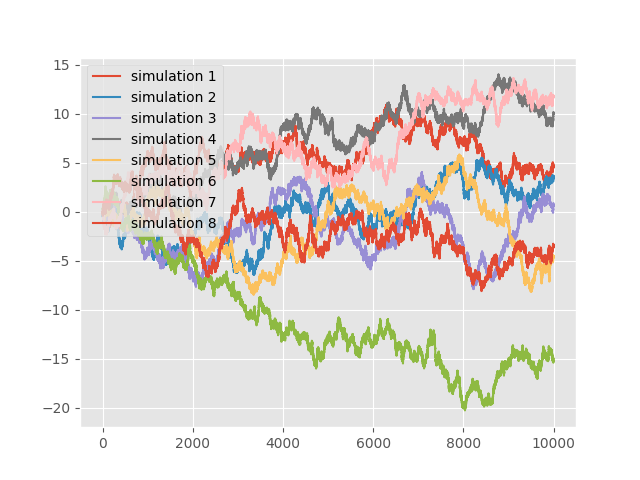
\includegraphics[width=1.5\linewidth]{bm_simulations.png}
\end{document}
